\chapter{Diskussion}

Hier wird reflektiert, in welchem Umfang die Zielsetzungen der Arbeit erreicht werden konnten. In der Regel gelingt dies durch den Bezug auf die Evaluation.

Typischer Umfang: 1-2 Seiten.

\section{Ausblick}

Manchmal konnte im Rahmen einer Bachelor- oder Masterarbeit ein
wissenschaftliches Thema auch so tief bearbeitet werden, dass wir es auf einem
wissenschaftlichen Workshop oder einer Konferenz veröffentlichen konnten.

Für Themen aus dem Bereich Virtuelle oder Erweiterte Realität bietet sich dazu
zum Beispiel der jährlich stattfindende Workshop der Fachgruppe VR/AR der
Gesellschaft für Informatik an. \citet{Bluhm:Sonar:2009} ist nur ein Beispiel
von mehreren Veröffentlichungen aus unserer Gruppe.

\section{Test}
Kleine Tests, die später noch passend in den übrigen Text eingearbeitet werden.

\subsection{Tabelle}

Das ist \autoref{tab:example}.

\begin{table}[tbh]
 \centering
 \begin{tabular}{r|r}
 Test 1 & Test 2\\
 \hline
 abc & 123\\
 def & 456\\
 ghi & 789
 \end{tabular}
 \caption{Tabellen-Test}
 \label{tab:example}
\end{table}

\subsection{Bild}

Das ist \autoref{fig:example}.

\begin{figure}[tbh]
 \centering
 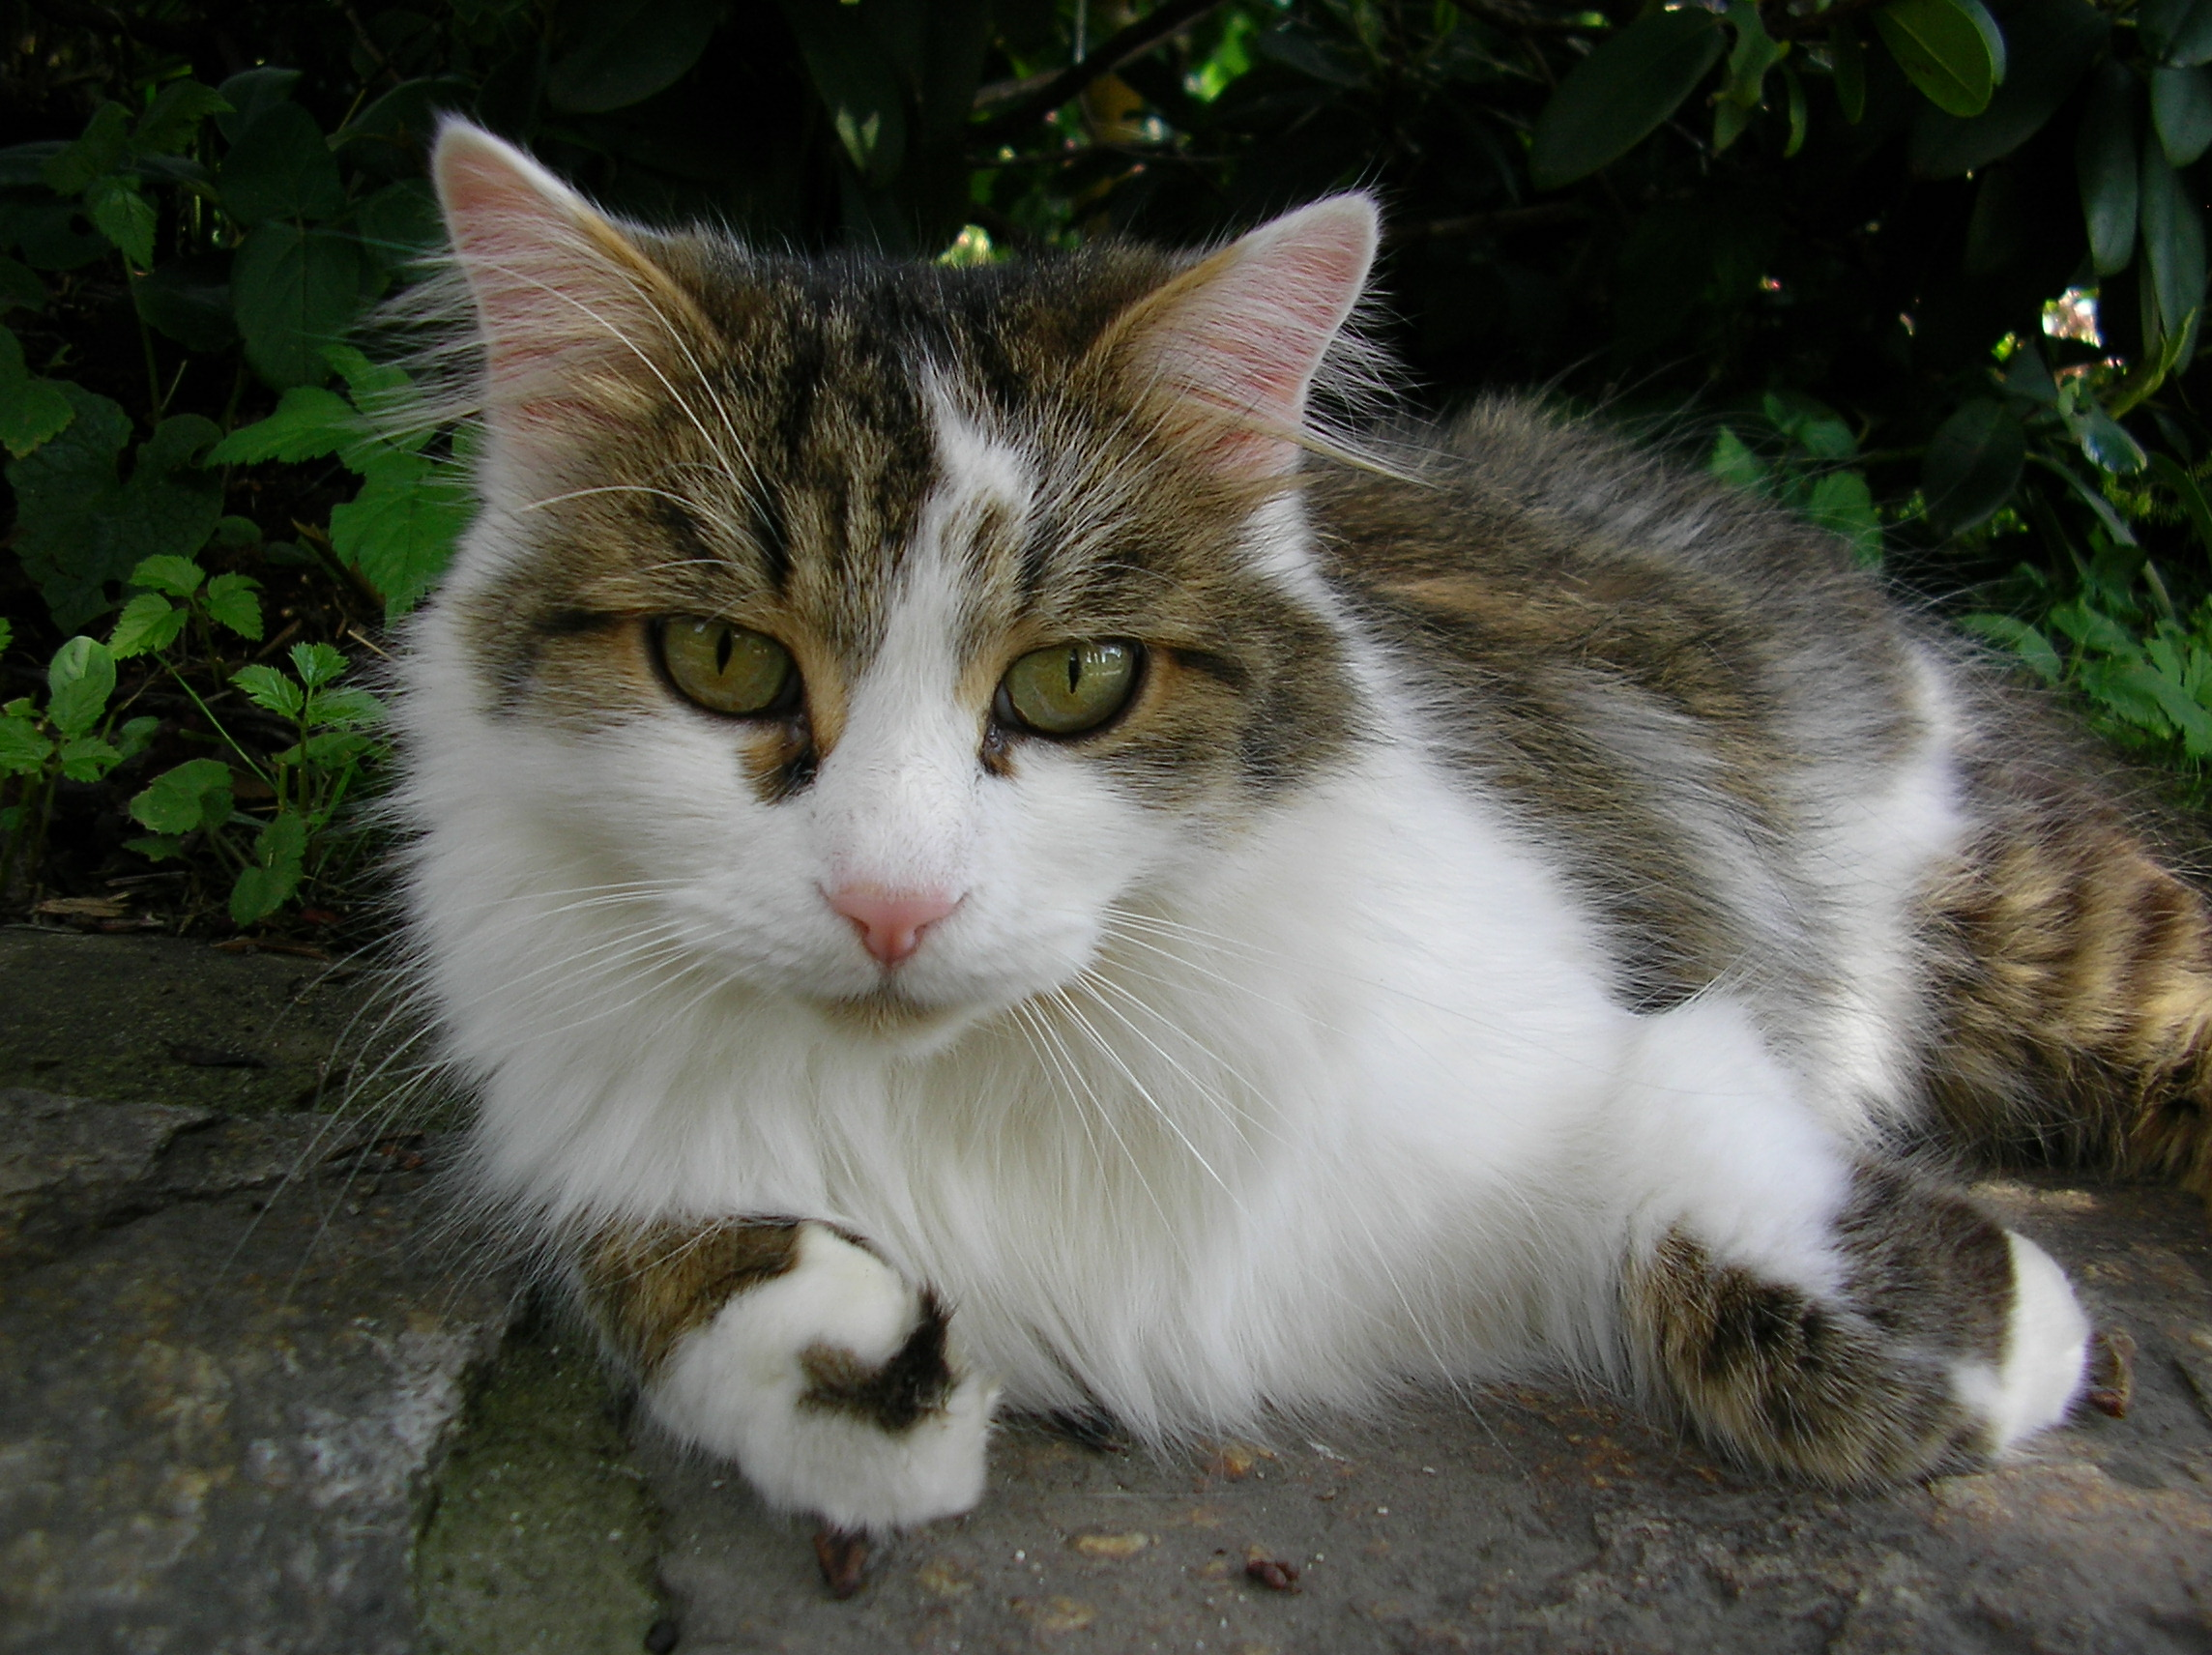
\includegraphics[width=0.5\textwidth]{Hauskatze_langhaar.jpg}
 \caption{Test-Bild}
 \label{fig:example}
\end{figure}

\subsection{Begriffe und Abkürzungen}
The \Gls{latex} typesetting markup language is specially suitable for documents that include \gls{maths}. \Glspl{formula} are rendered properly an easily once one gets used to the commands.

Given a set of numbers, there are elementary methods to compute its \acrlong{gcd}, which is abbreviated \acrshort{gcd}. This process is similar to that used for the \acrfull{lcm}.

\subsection{Mathematik}

\begin{equation}
 \sin \alpha = \left( \frac{a}{c} \right)
\end{equation}

\subsection{Code}

\autoref{lst:example} ist ein Code-Beispiel in Python.

\begin{lstlisting}[language=Python, caption=Code-Beispiel mit Python, label={lst:example}]
import numpy as np
    
def incmatrix(genl1,genl2):
    m = len(genl1)
    n = len(genl2)
    M = None #to become the incidence matrix
    VT = np.zeros((n*m,1), int)  #dummy variable
    
    #compute the bitwise xor matrix
    M1 = bitxormatrix(genl1)
    M2 = np.triu(bitxormatrix(genl2),1) 

    for i in range(m-1):
        for j in range(i+1, m):
            [r,c] = np.where(M2 == M1[i,j])
            for k in range(len(r)):
                VT[(i)*n + r[k]] = 1;
                VT[(i)*n + c[k]] = 1;
                VT[(j)*n + r[k]] = 1;
                VT[(j)*n + c[k]] = 1;
                
                if M is None:
                    M = np.copy(VT)
                else:
                    M = np.concatenate((M, VT), 1)
                
                VT = np.zeros((n*m,1), int)
    
    return M
\end{lstlisting}
